% OFDMA description and comparison with OFDM  
\section{What does OFDMA bring ?}
%
\indent OFDMA stands for \textit{Orthogonal Frequency Division Multiple Access}. It allows multiple users to communicate at the same time while keeping the high data rates offered by OFDM.\\
%
\indent The base principle of OFDMA consists in sharing the time and frequency resources between users. It can somehow be compared to a combination of OFDM, FDMA (\textit{Frequency Division Multiple Access}) and TDMA (\textit{Time Division Multiple Access})\cite{WikiOFDMA}. Users are assigned a subset of sub-carriers in the given frequency range and use it for a certain time before it is attributed to another user.\\
\indent All communications can happen in parallel and the attribution of sub-channels is made independently one from another : they can take place at different times and involve different size of sub-channels, see \figref{fig:OFDMvsOFDMA}.\\
%
\begin{figure}[H]
  \centering
  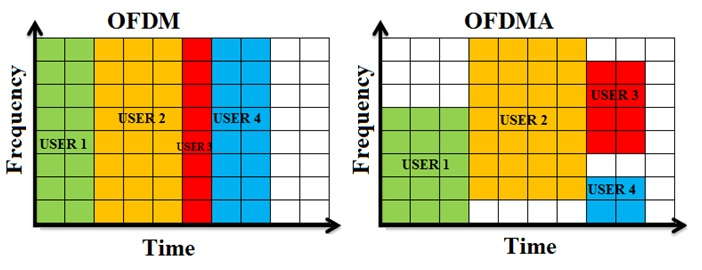
\includegraphics[width=\textwidth]{figures/difference-between-ofdm-and-ofdma.jpg}
  \caption{Comparison between OFDM and OFDMA \textbf{[source: differencebetween.com]}}
  \label{fig:OFDMvsOFDMA}
\end{figure}
%
\indent OFDMA still keeps a strong disadvantage from OFDM which is the high peak-to-power ratio which makes the use of this technique inefficient in terms of energy for small and portable devices. Despite this fact, OFDMA communication technique has been chosen for 4G LTE networks, designed especially for mobile communications (voice calls, video calls and streaming, World Wide Web access, ...). The next chapter explains briefly how this is achieved.

\paragraph*{See also,}
\cite[Chap.~19]{AMolisch}.